%=====================================================================
% Industrial Component Anomaly Detection – Defence Presentation
% Latex Beamer, 16:9
%=====================================================================
\documentclass[aspectratio=169,10pt]{beamer}

% ---- Theme ----
\usetheme{metropolis}
\usepackage{appendixnumberbeamer}
\usepackage{pgfpages}

% ---- Notes mode: compile with -jobname=notes to get presenter notes ----
% Activated externally by notes.tex via \def\NOTESMODE{1}
\ifdefined\NOTESMODE
  \setbeameroption{show only notes}
  \makeatletter
  \setbeamertemplate{note page}{%
    {%
      \scriptsize
      \usebeamerfont{note title}\usebeamercolor[fg]{note title}%
      \vbox{
        \hfill\insertslideintonotes{0.18}\hskip-\Gm@rmargin\hskip0pt%
        \vskip-0.18\paperheight%
        \nointerlineskip
        \begin{pgfpicture}{0cm}{0cm}{0cm}{0cm}
          \begin{pgflowlevelscope}{\pgftransformrotate{90}}
            {\pgftransformshift{\pgfpoint{-1.4cm}{0.2cm}}%
            \pgftext[base,left]{\usebeamerfont{note date}\usebeamercolor[fg]{note date}\the\year-\ifnum\month<10\relax0\fi\the\month-\ifnum\day<10\relax0\fi\the\day}}
          \end{pgflowlevelscope}
        \end{pgfpicture}}%
      \nointerlineskip
      \vbox to .18\paperheight{\vskip0.2em
        \hbox{\insertshorttitle[width=0.75\textwidth]}%
        \setbox\beamer@tempbox=\hbox{\insertsection}%
        \hbox{\ifdim\wd\beamer@tempbox>1pt{\hskip4pt\raise3pt\hbox{\vrule width0.4pt height7pt\vrule width 9pt height0.4pt}}\hskip1pt\hbox{\insertsection}\fi}%
        \setbox\beamer@tempbox=\hbox{\insertshortframetitle}%
        \hbox{\ifdim\wd\beamer@tempbox>1pt{\hskip16pt\raise3pt\hbox{\vrule width0.4pt height7pt\vrule width 9pt height0.4pt}}\hskip1pt\hbox{\insertshortframetitle}\fi}%
        \vfil}%
    }%
    \vskip.15em
    \nointerlineskip
    \insertnote
  }
  \makeatother
\fi

% Presenter note typography (compact size to prevent vertical overflow)
\newcommand{\notefont}{\fontsize{6.0pt}{7.2pt}\selectfont}

% ---- Packages ----
\usepackage{graphicx}
\usepackage{booktabs}
\usepackage{colortbl}
\usepackage{tabularx}
\usepackage{amsmath,amssymb}
\usepackage{xcolor}
\usepackage{tikz}
\usetikzlibrary{positioning,arrows.meta,shapes.geometric,fit,calc,backgrounds}
\usepackage{pgfplots}
\pgfplotsset{compat=1.18}
\usepackage{microtype}

\usepackage{hyperref}
\usepackage{multirow}
\usepackage{adjustbox}

% ---- Colours matching Streamlit deck ----
\definecolor{teal}{HTML}{007F7A}
\definecolor{accent}{HTML}{F06C54}
\definecolor{muted}{HTML}{6B7280}
\definecolor{lightbg}{HTML}{F7F6F3}
\definecolor{darkink}{HTML}{1A1A2E}
\definecolor{goodgreen}{HTML}{007F7A}
\definecolor{defectred}{HTML}{F06C54}

\setbeamercolor{frametitle}{fg=white, bg=teal}
\setbeamercolor{progress bar}{fg=accent}
\setbeamercolor{title separator}{fg=accent}
\setbeamercolor{alerted text}{fg=accent}
\setbeamercolor{example text}{fg=teal}

% ---- Figure paths ----
\graphicspath{
  {figures/defect_examples/}
  {figures/charts/}
  {figures/report_figures/}
  {figures/business/}
}

%=====================================================================
\title{Industrial Component Anomaly Detection}
\subtitle{Unsupervised defect classification and pixel-level anomaly\\
  localisation from normal-only manufacturing parts}
\author{Benjamin~Förster \and Ali~Abul~Hawa \and Mahboubeh~Nadaf \and Karim~Khalifa}
\date{September 2026}
\institute{Applied Machine Learning · MVTec AD Benchmark}
%=====================================================================

\begin{document}

%--------------------------------------------------------------------
% SLIDE 1 – TITLE
%--------------------------------------------------------------------
\newcommand{\pilltag}[1]{%
  \tikz[baseline=-0.6ex]\node[fill=teal!15, rounded corners=2pt, inner sep=3pt, font=\tiny\bfseries\color{teal}]{#1};%
}
\newcommand{\thumb}[3]{% #1=filename, #2=badge-color, #3=badge-text
  \tikz[baseline=(img.south)]{%
    \node[inner sep=0] (img) {\includegraphics[width=1.7cm,height=1.7cm,keepaspectratio]{#1}};%
    \node[fill=#2, text=white, font=\tiny\bfseries, inner sep=1.5pt, anchor=south west] at (img.south west) {#3};%
  }%
}
\newcommand{\goodimg}[1]{\thumb{#1}{goodgreen}{GOOD}}
\newcommand{\defectimg}[1]{\thumb{#1}{defectred}{DEFECT}}

% --- Slide Frame ---
\begin{frame}[plain]
\begin{columns}[T, onlytextwidth]

  % Left column: Title & Context
  \begin{column}{0.60\textwidth}
    \vspace*{0.6cm}
    {\large\bfseries\color{darkink} Industrial Component\\[2pt] Anomaly Detection}\\[4pt]
    {\small\color{accent} Project Presentation}\\[6pt]
    \rule{3.2cm}{1.2pt}\\[6pt]
    {\footnotesize\color{darkink}
      Unsupervised defect classification and pixel-level anomaly localisation from normal-only manufacturing parts.}\\[8pt]
    \pilltag{Unsupervised AD} \pilltag{Deep Transfer Learning} \pilltag{Zero-Leakage Protocol}\\[10pt]
    {\tiny\bfseries\color{muted} TEAM}\\[2pt]
    {\footnotesize\color{muted}
      B. Förster $\cdot$ A. Abul Hawa $\cdot$ M. Nadaf $\cdot$ K. Khalifa}
  \end{column}

  % Right column: Image showcase table
  \begin{column}{0.42\textwidth}
    \vspace*{0.3cm}
    {\tiny\bfseries\color{muted} MVTEC AD 2D Dataset \hfill \color{teal}Selected Examples $\cdot$ Objects \& Textures}\\[4pt]
    
    % \resizebox guarantees the table fits the column width exactly
    \resizebox{1\linewidth}{!}{%
      \setlength{\tabcolsep}{3pt}%
      \begin{tabular}{@{} lcc @{}}
        \tiny\bfseries\color{muted} CATEGORY & \tiny\bfseries\color{muted} CONFORMING & \tiny\bfseries\color{muted} DEFECTIVE \\[3pt]
        \textbf{Bottle}\newline{\footnotesize\color{muted}$\quad$ Broken rim}    & \goodimg{title_good_bottle.png}  & \defectimg{title_anomaly_bottle.png}  \\[3pt]
        \textbf{Capsule}\newline{\footnotesize\color{muted}$\quad$ Scratch}      & \goodimg{title_good_capsule.png} & \defectimg{title_anomaly_capsule.png} \\[3pt]
        \textbf{Leather}\newline{\footnotesize\color{muted}$\quad$ Surface cut}  & \goodimg{title_good_leather.png} & \defectimg{title_anomaly_leather.png} \\[3pt]
        \textbf{Screw}\newline{\footnotesize\color{muted}$\quad$ Thread defect}  & \goodimg{title_good_screw.png}   & \defectimg{title_anomaly_screw.png}   \\
      \end{tabular}%
    }
  \end{column}

\end{columns}
\end{frame}

%====================================================================
%  SECTION: DATA EXPLORATION
%====================================================================
\section{Data Exploration}

%--------------------------------------------------------------------
% SLIDE 2 – MVTec AD Dataset & Class Imbalance
%--------------------------------------------------------------------
\begin{frame}{The MVTec AD Dataset -- Class Imbalance}
\begin{columns}[T]
  \begin{column}{0.55\textwidth}
    \textbf{Dataset at a glance}
    \begin{itemize}\small
      \item 15 manufacturing categories: 10 objects + 5 textures
      \item $> 5000$ images,  $\approx 1200$ anomalous images
      \item Normal-only training; test set has pixel-level anomaly ground truth
    \end{itemize}
    \textbf{\color{accent}Accuracy paradox}
    \begin{itemize}
      \item Median anomalous-pixel area: \textbf{1.54\%}
      \item Predicting \emph{all-normal} yields $>$98.5\% pixel accuracy while catching \emph{zero} defects.
    \end{itemize}
    \textbf{Kruskal-Wallis: $H(14)\approx626.5$, $p<0.001$}
    \begin{itemize}
      \item 43$\times$ spread in defect size across categories.
    \end{itemize}
  \end{column}
  \begin{column}{0.31\textwidth}
    \begin{center}
      {\tiny\bfseries\color{muted} TEST-SET CLASS IMBALANCE (images)}\\[3pt]
      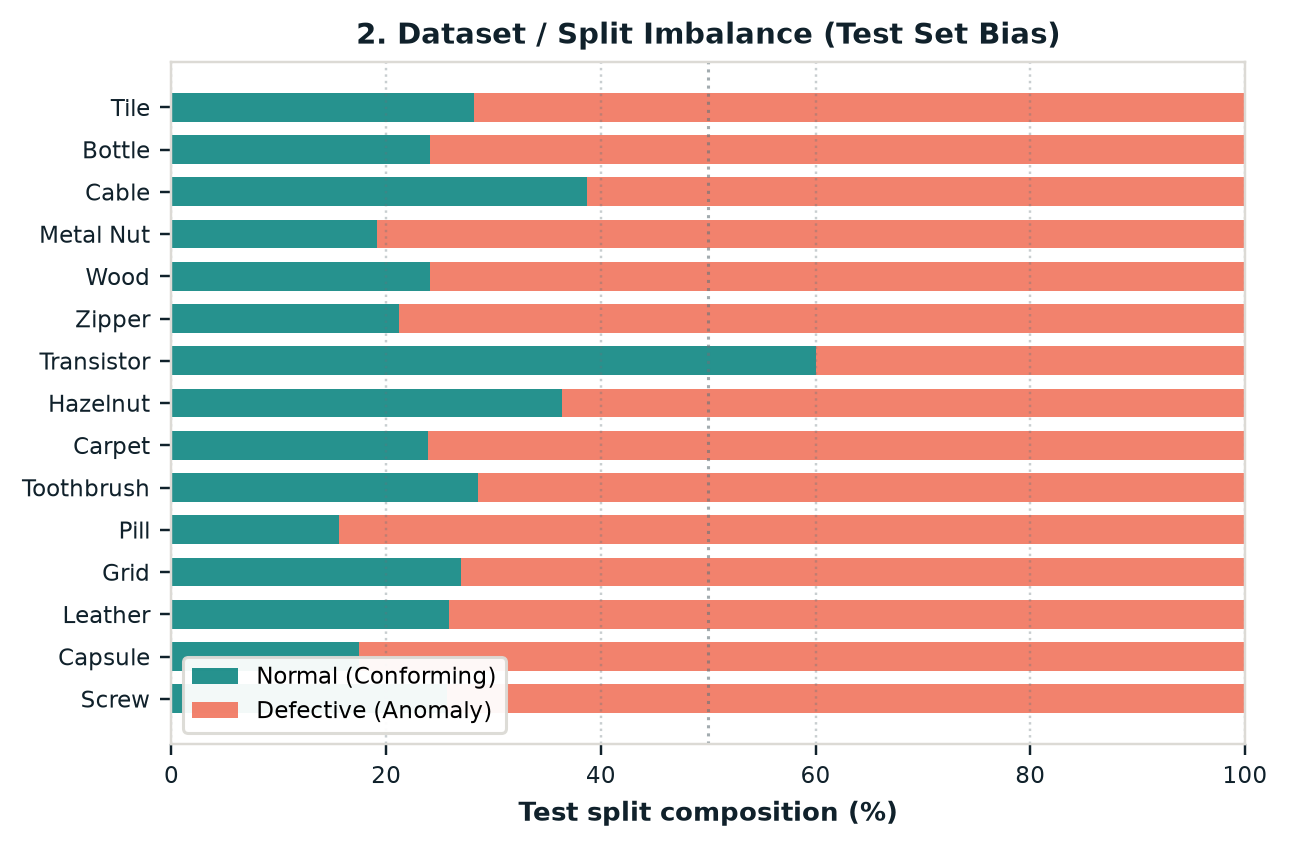
\includegraphics[width=\textwidth,height=0.68\textheight,keepaspectratio]{imbalance_test_split.png}
    \end{center}
    \vspace{-0.5cm}
    \begin{center}
      {\tiny\bfseries\color{muted} PIXEL-AREA IMBALANCE (defect region \%)}\\[3pt]
      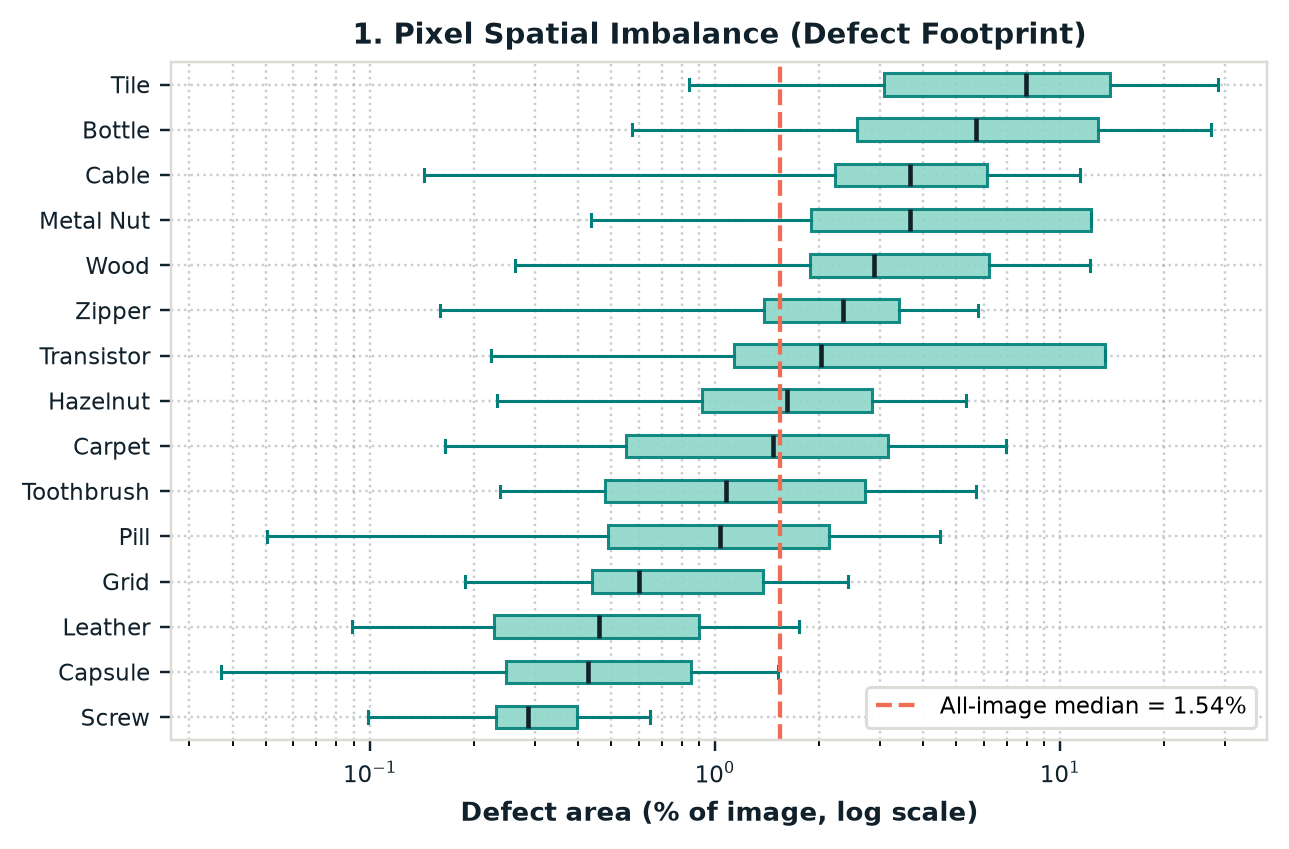
\includegraphics[width=\textwidth,height=0.68\textheight,keepaspectratio]{imbalance_pixel_area.png}
    \end{center}
  \end{column}
\end{columns}
\end{frame}

%--------------------------------------------------------------------
% SLIDE 3 – Defect Taxonomy & Spatial Distribution
%--------------------------------------------------------------------
\begin{frame}{Defect Taxonomy \& Spatial Distribution}
\begin{columns}[T]
  \begin{column}{0.55\textwidth}
    \textbf{Two fundamentally different defect regimes:}\\[6pt]
    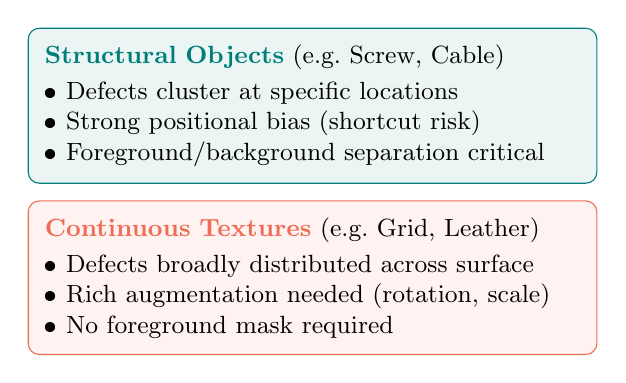
\begin{tikzpicture}[font=\small]
      \node[draw=teal,rounded corners,fill=teal!8,text width=6.8cm,inner sep=6pt] (obj) {
        \textbf{\color{teal}Structural Objects} (e.g.\ Screw, Cable)\\[2pt]
        \textbullet\ Defects cluster at specific locations\\
        \textbullet\ Strong positional bias (shortcut risk)\\
        \textbullet\ Foreground/background separation critical
      };
      \node[draw=accent,rounded corners,fill=accent!8,text width=6.8cm,inner sep=6pt,below=6pt of obj] (tex) {
        \textbf{\color{accent}Continuous Textures} (e.g.\ Grid, Leather)\\[2pt]
        \textbullet\ Defects broadly distributed across surface\\
        \textbullet\ Rich augmentation needed (rotation, scale)\\
        \textbullet\ No foreground mask required
      };
    \end{tikzpicture}
    \vspace{6pt}\\
    \textbf{Covariate shift:} Screw, Leather, Grid show measurable
    brightness/contrast drift between train and test normal images --
    motivates photometric augmentation.
  \end{column}
  \begin{column}{0.42\textwidth}
    \begin{center}
    {\tiny\bfseries\color{teal} OBJECTS -- LOCALISED DEFECTS (contour = defect boundary)}\\[4pt]
    \setlength{\tabcolsep}{3pt}
    \begin{tabular}{ccc}
      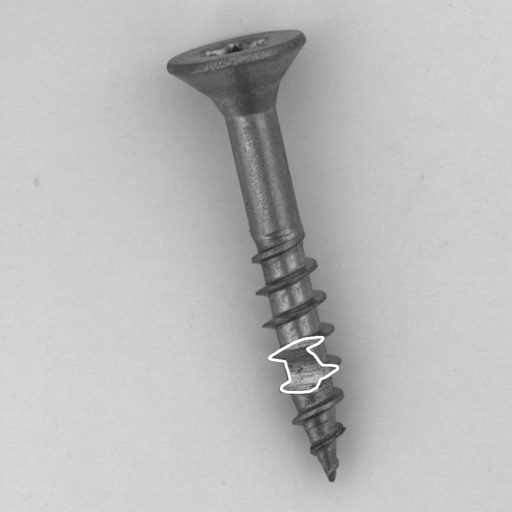
\includegraphics[width=1.7cm,keepaspectratio]{slide_03_screw_thread_contour.png} &
      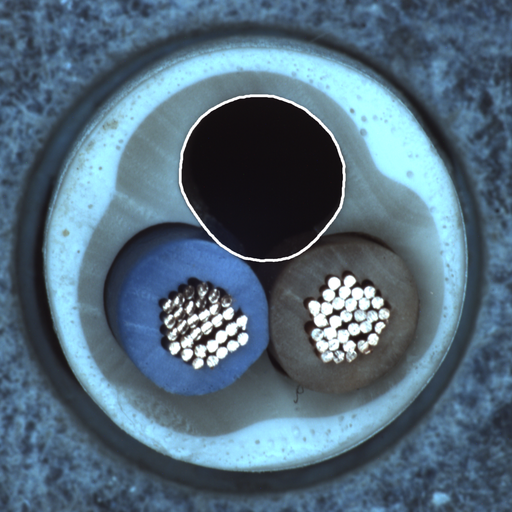
\includegraphics[width=1.7cm,keepaspectratio]{slide_03_cable_missing_contour.png} &
      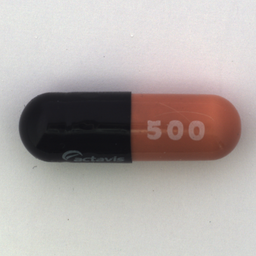
\includegraphics[width=1.7cm,keepaspectratio]{title_anomaly_capsule.png} \\
      {\tiny\color{muted} Screw thread} &
      {\tiny\color{muted} Cable missing} &
      {\tiny\color{muted} Capsule scratch} \\[4pt]
    \end{tabular}
    {\tiny\bfseries\color{accent} TEXTURES -- DISTRIBUTED DEFECTS (defect across full surface)}\\[4pt]
    \begin{tabular}{ccc}
      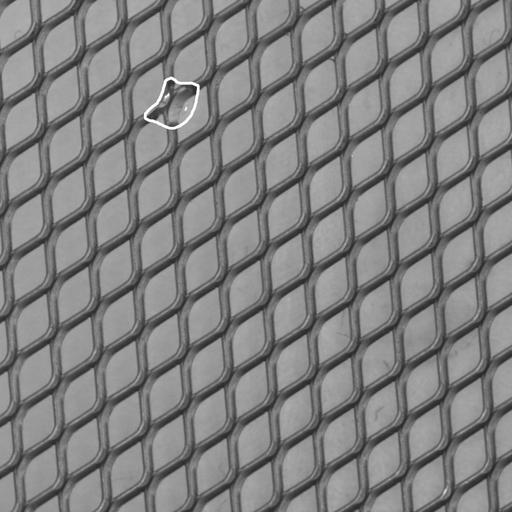
\includegraphics[width=1.7cm,keepaspectratio]{slide_03_grid_glue_contour.png} &
      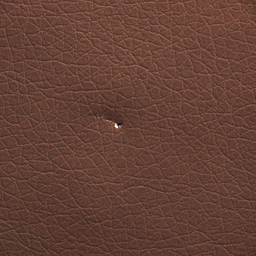
\includegraphics[width=1.7cm,keepaspectratio]{title_anomaly_leather.png} &
      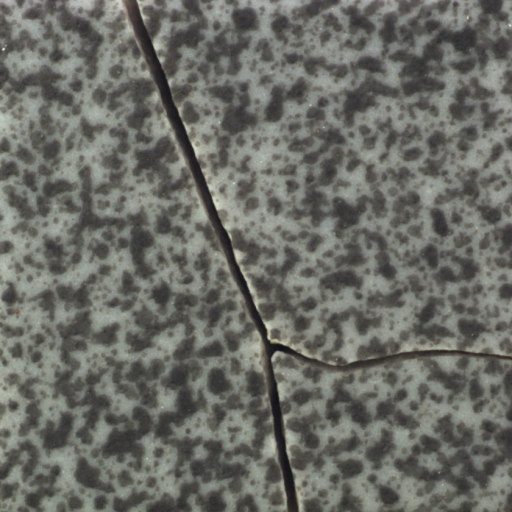
\includegraphics[width=1.7cm,keepaspectratio]{slide_03_tile_crack.png} \\
      {\tiny\color{muted} Grid glue strip} &
      {\tiny\color{muted} Leather cut} &
      {\tiny\color{muted} Tile crack} \\
    \end{tabular}
    \end{center}
  \end{column}
\end{columns}
\end{frame}


%--------------------------------------------------------------------
% SLIDE 4 – Metric Selection
%--------------------------------------------------------------------
\begin{frame}{Metric Selection: AUPIMO \& F1-Score}
\begin{columns}[T]
  \begin{column}{0.58\textwidth}
    \textbf{\color{accent}The Problem with Pixel-AUROC}
    \begin{itemize}\small
      \item AUROC relies on False Positive Rate (FPR):
      \begin{itemize}\footnotesize
        \item With $\approx$\,98.5\% normal pixels, TN dominates $\Rightarrow$ FPR barely moves.
        \item SOTA scores all exceed 99\%, making differences indistinguishable.
      \end{itemize}
    \end{itemize}
    \vspace{3pt}
    \textbf{\color{teal}Metric Solution}
    \begin{itemize}\small
      \item \textbf{AUPIMO:} Integrates localization over the operational ultra-low FPR window $[10^{-5}, 10^{-4}]$ on normal images.
      \item \textbf{Dual Thresholds:} We calibrate distinct \emph{image-level} and \emph{pixel-level} anomaly thresholds.
      \item \textbf{F1-Score / PR Curve:} Directly measures defect capture vs false alarms without TN dilution.
    \end{itemize}
  \end{column}
  \begin{column}{0.40\textwidth}
    \centering
    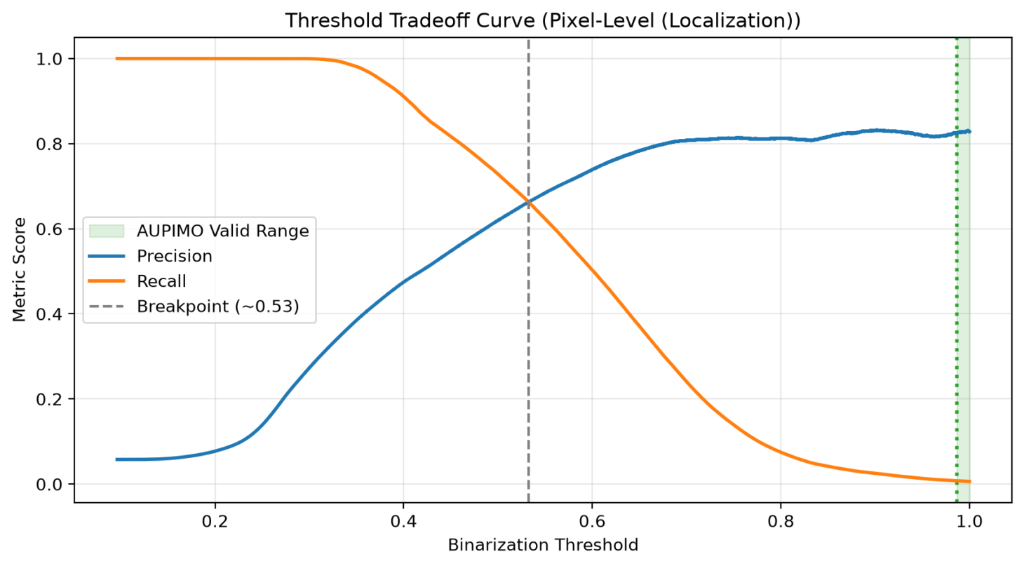
\includegraphics[width=\textwidth]{binarization_threshold_aupimo.png}\\[-6pt]
    {\tiny\color{muted} Threshold tradeoff curve \& AUPIMO range}\\[3pt]
    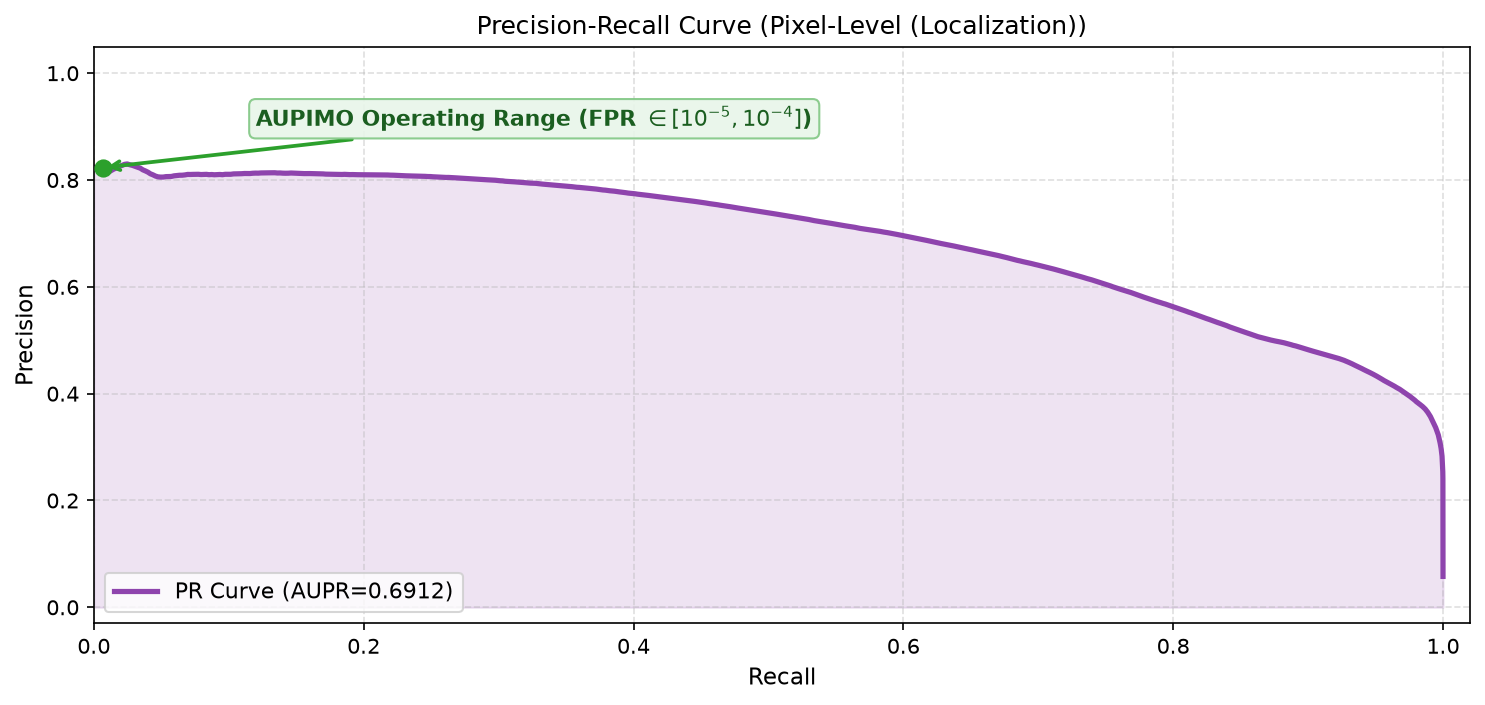
\includegraphics[width=\textwidth]{pr_curve_aupimo.png}\\[-6pt]
    {\tiny\color{muted} Precision-Recall curve with marked AUPIMO operating range}\par
  \end{column}
\end{columns}
\end{frame}

%====================================================================
%  SECTION: MODELS
%====================================================================
\section{Models}

%--------------------------------------------------------------------
% SLIDE 5 – Model Selection & Architecture Overview
%--------------------------------------------------------------------
\begin{frame}{Model Selection \& Architecture Overview}
\vspace*{-0.2cm}
\begin{columns}[T, onlytextwidth]

  %=========================================
  % Left Column: Custom Conv-Autoencoders
  %=========================================
  \begin{column}{0.48\textwidth}
    \begin{block}{\small\bfseries 1. Convolutional-Autoencoders}
      \vspace{2pt}
      {\tiny\color{muted}\textbf{Paradigm:} Generative Reconstruction $\cdot$ Built from scratch}\\[4pt]
      
      \centering
      \resizebox{0.95\linewidth}{!}{
        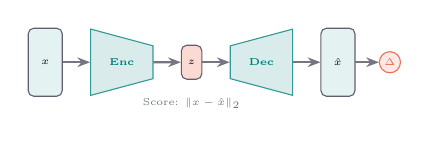
\begin{tikzpicture}[
  scale=0.72, every node/.style={scale=0.72},
  block/.style={draw=darkink!70, fill=white, rounded corners=2pt, minimum height=1.2cm, align=center, font=\tiny},
  arr/.style={-{Stealth[scale=0.7]}, thick, color=darkink!60}
]
  % Input
  \node[block, minimum width=0.6cm, fill=teal!10] (in) {$x$};
  
  % Encoder (Trapezoid)
  \node[draw=teal!80, fill=teal!15, shape=trapezium, shape border rotate=270, 
        minimum height=1.1cm, trapezium angle=75, right=0.35cm of in, font=\tiny\bfseries\color{teal}] (enc) {Enc};
  
  % Bottleneck
  \node[block, right=0.35cm of enc, minimum width=0.25cm, minimum height=0.6cm, fill=accent!25] (z) {\tiny $z$};
  
  % Decoder (Trapezoid)
  \node[draw=teal!80, fill=teal!15, shape=trapezium, shape border rotate=90, 
        minimum height=1.1cm, trapezium angle=75, right=0.35cm of z, font=\tiny\bfseries\color{teal}] (dec) {Dec};
  
  % Output & Error
  \node[block, minimum width=0.6cm, fill=teal!10, right=0.35cm of dec] (out) {$\hat{x}$};
  \node[draw=defectred, fill=defectred!15, circle, inner sep=1.5pt, right=0.3cm of out, font=\tiny\bfseries\color{defectred}] (diff) {$\Delta$};

  % Arrows
  \draw[arr] (in) -- (enc);
  \draw[arr] (enc) -- (z);
  \draw[arr] (z) -- (dec);
  \draw[arr] (dec) -- (out);
  \draw[arr] (out) -- (diff);
  
  % Bottom note
  \node[below=0.15cm of z, font=\tiny\color{muted}] {Score: $\|x - \hat{x}\|_2$};
\end{tikzpicture}

      }
      \vspace{2pt}
    \end{block}

    \vspace{4pt}
    {\small
    \begin{itemize}\setlength{\itemsep}{2pt}\setlength{\leftskip}{-10pt}
      \item \textbf{Complete control:} Full freedom over latent bottleneck dimensions, skip connections, and loss constraints.
      \item \textbf{Intuition:} Trained on normal images; unable to reconstruct defects.
      \item \textbf{Trade-offs:} Prone to blurriness or identity shortcuts; sensitive to reconstruction thresholds.
    \end{itemize}
    }
  \end{column}

  %=========================================
  % Right Column: PatchCore + ResNet-18
  %=========================================
  \begin{column}{0.48\textwidth}
    \begin{block}{\small\bfseries 2. PatchCore + ResNet-18 (Anomalib)}
      \vspace{2pt}
      {\tiny\color{muted}\textbf{Paradigm:} Deep Feature Memory Bank $\cdot$ High accessibility}\\[4pt]
      
      \centering
      \resizebox{0.88\linewidth}{!}{
        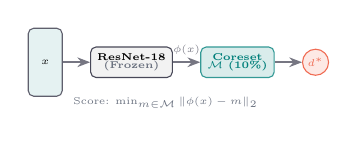
\begin{tikzpicture}[
  scale=0.72, every node/.style={scale=0.72},
  block/.style={draw=darkink!70, fill=white, rounded corners=2pt, minimum height=1.2cm, align=center, font=\tiny},
  arr/.style={-{Stealth[scale=0.7]}, thick, color=darkink!60}
]
  % Input Image
  \node[block, minimum width=0.6cm, fill=teal!10] (p_in) {$x$};
  
  % Backbone
  \node[draw=darkink!80, fill=black!5, rounded corners=2pt, right=0.35cm of p_in, 
        minimum width=1.1cm, align=center, font=\tiny\bfseries] (bb) {ResNet-18\\[-2pt]{\tiny\color{muted}(Frozen)}};
  
  % Memory Bank / Coreset
  \node[draw=teal!80, fill=teal!15, rounded corners=2pt, right=0.35cm of bb, 
        minimum width=0.9cm, align=center, font=\tiny\bfseries\color{teal}] (mem) {Coreset\\[-2pt]{\tiny $\mathcal{M}$ (10\%)}};
  
  % k-NN Match
  \node[draw=defectred, fill=defectred!15, circle, inner sep=1.5pt, right=0.35cm of mem, 
        font=\tiny\bfseries\color{defectred}] (knn) {$d^*$};

  % Arrows
  \draw[arr] (p_in) -- (bb);
  \draw[arr] (bb) -- node[above, font=\tiny] {$\phi(x)$} (mem);
  \draw[arr] (mem) -- (knn);

  % Bottom note
  \node[below=0.15cm of bb, font=\tiny\color{muted}, xshift=0.6cm] {Score: $\min_{m \in \mathcal{M}} \|\phi(x) - m\|_2$};
\end{tikzpicture}

      }
      \vspace{2pt}
    \end{block}

    \vspace{-4pt}
    {\small
    \begin{itemize}\setlength{\itemsep}{2pt}\setlength{\leftskip}{-10pt}
      \item \textbf{High accessibility:} Zero model training required; out-of-the-box integration via Intel's \texttt{anomalib}.
      \item \textbf{ResNet-18 backbone:} Compact ImageNet representations; mid-level layers capture both texture and shape.
      \item \textbf{Coreset sampling:} Compresses the memory bank by 90\%+ without losing local anomaly detection accuracy.
    \end{itemize}
    }
  \end{column}

\end{columns}
\note{\notefont
  \textbf{Notation on PatchCore diagram ($\phi(x)$ and $m \in \mathcal{M}$):}\\[0.5pt]
  $\phi(x)$ is the \emph{patch feature representation} extracted from frozen ResNet-18 (concatenated mid-level layers 2+3).
  $\mathcal{M}$ is the \emph{coreset memory bank} of normal reference vectors, and $m \in \mathcal{M}$ is an individual stored normal patch prototype.
  $\min_{m \in \mathcal{M}} \|\phi(x) - m\|_2$ is the nearest-neighbour $L_2$ distance: an anomaly is detected when a query patch vector has no close normal counterpart in memory.\\[1.5pt]

  \textbf{Q: Why two such different paradigms rather than one?}\\[0.5pt]
  They fail in completely different ways. A CAE can fail silently on textures it has never seen,
  while PatchCore fails when the memory bank has coverage gaps. Running both gives orthogonal error signals.
  PatchCore is also a natural upper-bound baseline: if PatchCore cannot detect a defect with frozen
  ImageNet features, the defect has near-zero visual contrast — no learned model will either.\\[1.5pt]

  \textbf{Q: Couldn't you just use a classifier with defect labels?}\\[0.5pt]
  Hard no in industrial production: defect labels require defective parts to exist,
  which means letting defective parts accumulate before deployment. The whole value proposition
  is Day-1 deployment with zero defect data. Any supervised approach also fails on
  \emph{novel} defect types not seen during training.\\[1.5pt]

  \textbf{Conceptual trap: PatchCore ``trains'' vs.~``fits''.}\\[0.5pt]
  PatchCore has no gradient updates. The ``fitting'' step is just a forward pass through
  ResNet-18 + writing vectors to memory. The distinction matters: there is no overfitting risk,
  no learning rate to tune, no epochs. It is closer to database indexing than training.\\[1.5pt]

  \textbf{Connection between models:} Both ultimately compute a per-patch distance to normality
  — CAE in pixel reconstruction space, PatchCore in feature embedding space.
  The difference is \emph{where} normal is represented: CAE encodes it in weights, PatchCore in vectors.
}
\end{frame}

%--------------------------------------------------------------------
% SLIDE 6 – PatchCore: Transfer Learning \& Architecture
%--------------------------------------------------------------------
\begin{frame}{PatchCore: Transfer Learning \& Architecture}
\begin{columns}[T]
  % Left Column: Flowchart
  \begin{column}{0.38\textwidth}
    \vspace{0.5cm}
    \centering
    \textbf{Transfer Learning Paradigm}\\[8pt]
    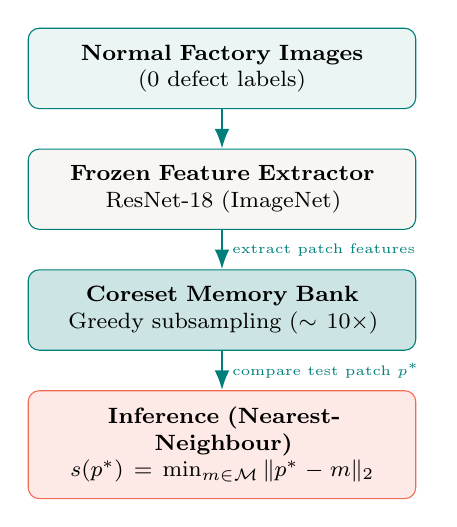
\begin{tikzpicture}[
      font=\footnotesize,
      box/.style={draw,rounded corners=4pt,text width=4.5cm,align=center,inner sep=6pt,minimum height=0.8cm},
      arr/.style={-{Latex[length=2.5mm]},thick,color=teal}
    ]
      \node[box,fill=teal!8,draw=teal] (normal) at (0,0) {\textbf{Normal Factory Images}\\(0 defect labels)};
      \node[box,fill=lightbg,draw=teal,below=0.5cm of normal] (frozen) {\textbf{Frozen Feature Extractor}\\ResNet-18 (ImageNet)};
      \node[box,fill=teal!20,draw=teal,below=0.5cm of frozen] (memory) {\textbf{Coreset Memory Bank}\\Greedy subsampling ($\sim10\times$)};
      \node[box,fill=accent!15,draw=accent,below=0.5cm of memory] (infer) {\textbf{Inference (Nearest-Neighbour)}\\$s(p^*)=\min_{m\in\mathcal{M}}\|p^*-m\|_2$};

      \draw[arr] (normal) -- (frozen);
      \draw[arr] (frozen) -- node[right,font=\tiny\color{muted}]{extract patch features} (memory);
      \draw[arr] (memory) -- node[right,font=\tiny\color{muted}]{compare test patch $p^*$} (infer);
    \end{tikzpicture}
  \end{column}

  % Right Column: Heatmaps & Description
  \begin{column}{0.6\textwidth}
    \begin{center}
      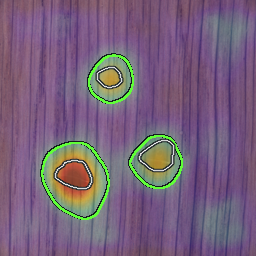
\includegraphics[width=0.24\linewidth]{slide_06_wood_liquid.png}\hfill
      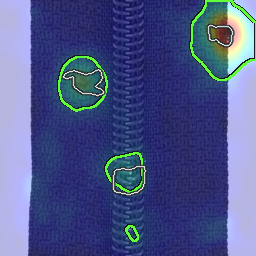
\includegraphics[width=0.24\linewidth]{slide_06_zipper_combined.png}\hfill
      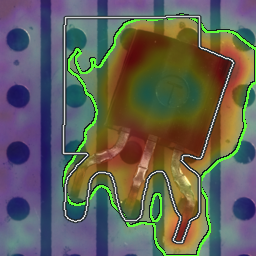
\includegraphics[width=0.24\linewidth]{slide_06_transistor_misplaced.png}\hfill
      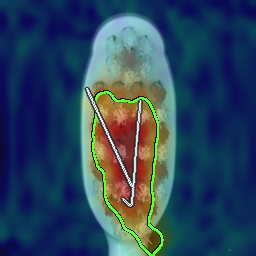
\includegraphics[width=0.24\linewidth]{slide_06_toothbrush_defective.png}
    \end{center}
    \vspace{-0.2cm}
    {\scriptsize\color{muted}\centering Wood, zipper, transistor, toothbrush. White = GT; green = predicted mask (pixel $q_{0.99}$).\par}
    \vspace{0.3cm}
    
    \footnotesize\textbf{Key Features}
    \begin{itemize}
      \item \textbf{Cold-start eliminated:} Deployment without defect collection.
      \item \textbf{IP Protection:} Memory bank contains embeddings, not raw model weights.
    \end{itemize}

    \textbf{\color{teal}Why it excels}
    \begin{itemize}
      \item Mid-level layers capture local textures perfectly.
      \item No catastrophic forgetting (frozen backbone).
      \item ResNet-18 guarantees predictable GPU memory bounds.
    \end{itemize}
  \end{column}
\end{columns}
\note{\notefont
  \textbf{Inference formula ($s(p^*) = \min_{m \in \mathcal{M}} \|p^* - m\|_2$):}\\[0.5pt]
  $p^* \equiv \phi(x)_i$ is the query patch feature vector extracted by frozen ResNet-18 $\phi(x)$.
  $\mathcal{M}$ is the coreset-reduced memory bank of normal training vectors, and $m \in \mathcal{M}$ is the nearest normal reference vector.
  Scoring is non-parametric nearest-neighbour distance: if a query patch has no close match in $\mathcal{M}$, its distance is large $\Rightarrow$ anomalous.\\[1.5pt]

  \textbf{Q: Why not fine-tune ResNet on the normal images?}\\[0.5pt]
  Without defect labels you can only do self-supervised fine-tuning. But this risks
  \emph{destroying} the mid-level texture representations that make PatchCore work
  — fine-tuning on a narrow distribution (one factory category) collapses the embedding
  space to only what it has seen, killing generalisation to subtle defects.
  The frozen features generalise better precisely because they were trained on 1M diverse images.\\[1.5pt]

  \textbf{Q: Why layer2+layer3 of ResNet-18 and not the final layer?}\\[0.5pt]
  The final layer encodes ImageNet class identity (cat, truck, etc.) — totally irrelevant
  to surface defects. Layer2/3 encode mid-level statistics: edges, frequency responses,
  local texture gradients. These are universal and transfer well to any visual texture domain.\\[1.5pt]

  \textbf{Q: How does coreset subsampling work without losing coverage?}\\[0.5pt]
  Greedy farthest-point sampling: iteratively pick the point in feature space that is
  farthest from all already-selected points. This guarantees maximum coverage of the
  feature space manifold with the fewest points. It is \emph{not} random subsampling.
  Random subsampling at 10\% would cluster around dense regions, leaving sparse regions
  (rare but valid normal appearances) uncovered — producing false positives.\\[1.5pt]

  \textbf{Failure mode to know:} PatchCore cannot detect defects that are \emph{globally}
  anomalous but locally normal. Example: a correct screw thread in the wrong location.
  Every individual patch looks fine; only the global arrangement is wrong.
  CAE is actually better here because it reconstructs the whole image.
}
\end{frame}


%--------------------------------------------------------------------
% SLIDE 7 – Keras CAE Learning Process
%--------------------------------------------------------------------
\begin{frame}{Keras CAE -- Autoencoder Learning Process}
\begin{columns}[T]
  \begin{column}{0.48\textwidth}
    {\small
    \textbf{\color{teal} The Concept}\\[8pt]
    
    \textbf{Training Phase:}
    \begin{itemize}
      \item Trained \emph{excl.} on defect-free images.
      \item Learns the structural grammar of "normal" surfaces.
    \end{itemize}
    
    \textbf{Inference Phase:}
    \begin{itemize}
      \item On defective images, anomalies are reconstructed as "normal" parts.
      \item Reconstruction fails at the defect sites $\Rightarrow$ high reconstruction error.
      \item High reconstruction error $\Rightarrow$ Anomaly Signal.
    \end{itemize}
    }
  \end{column}

  \begin{column}{0.48\textwidth}
    \textbf{\color{teal}Key Design Decisions}\\[6pt]
    {\small
    \begin{itemize}\setlength{\itemsep}{6pt}\setlength{\leftskip}{-10pt}
      \item \textbf{Masked Image Modelling (MIM):}\\
            25\% of patches randomly masked before encoding. Forces the model to understand global context, prevents "identity mapping".
      \item \textbf{SSIM + MSE Loss:}\\
            $\mathcal{L} = \alpha\,(1-\mathrm{SSIM}) + (1-\alpha)\,\mathrm{MSE}$.\\
            MSE captures global variance, while SSIM enforces high structural and perceptual fidelity.
      \item \textbf{Architectural Choices:}\\
            \textbf{ELU} no dying neurons + zero-centered mean.\\
            \textbf{BatchNorm} stabilizes covariate shifts.\\
            \textbf{AdamW} enables decoupled weight decay.
    \end{itemize}
    }
  \end{column}
\end{columns}
\note{\notefont
  \textbf{Q: Isn't the loss the anomaly score? (Classic confusion)}\\[0.5pt]
  No. The loss is a global image scalar used only during training for weight updates.
  The anomaly score is a \emph{per-pixel} error map aggregated via Top-K pooling, computed only
  at inference with frozen weights. They share the MSE signal but serve completely different purposes.
  The loss cannot localise defects; the pixel error map can.\\[1.5pt]

  \textbf{Q: Why does a decoder trained on normals fail on defects? It still has all its weights.}\\[0.5pt]
  The bottleneck is a learned \emph{normal manifold}. A defective image gets projected
  onto the closest point on that manifold, which is a normal surface. The decoder then
  faithfully decodes \emph{that projection}, not the original defective input.
  Think of it as a lossy codec trained only on one class: it always outputs something class-like.\\[1.5pt]

  \textbf{Q: Why SSIM and not just MSE?}\\[0.5pt]
  MSE optimises average pixel intensity independently — a blurry reconstruction can have
  low MSE. SSIM penalises structural differences: contrast, luminance, and local co-movement
  of pixels. A blur that preserves colour but destroys edges is heavily penalised by SSIM,
  not by MSE. The combination forces the reconstruction to be both globally correct (MSE)
  and structurally faithful (SSIM), which matters for texture surfaces like leather or wood.\\[1.5pt]

  \textbf{Q: Why not skip connections like a U-Net?}\\[0.5pt]
  Skip connections let the encoder pass high-frequency detail directly to the decoder,
  bypassing the bottleneck. This makes it \emph{trivially easy} to reconstruct any input,
  including defects. The bottleneck \emph{must} be the information bottleneck.
  MIM reinforces this: if you mask 25\% of the input, skip connections cannot carry
  the masked content, forcing the bottleneck to infer it from context.
}
\end{frame}

%--------------------------------------------------------------------
% SLIDE 8 – Keras CAE Pipeline (End-to-End)
%--------------------------------------------------------------------
\begin{frame}{Keras CAE -- End-to-End Pipeline}
\vspace*{-0.3cm}
\begin{center}
% codespell:disable
\resizebox{0.95\textwidth}{!}{
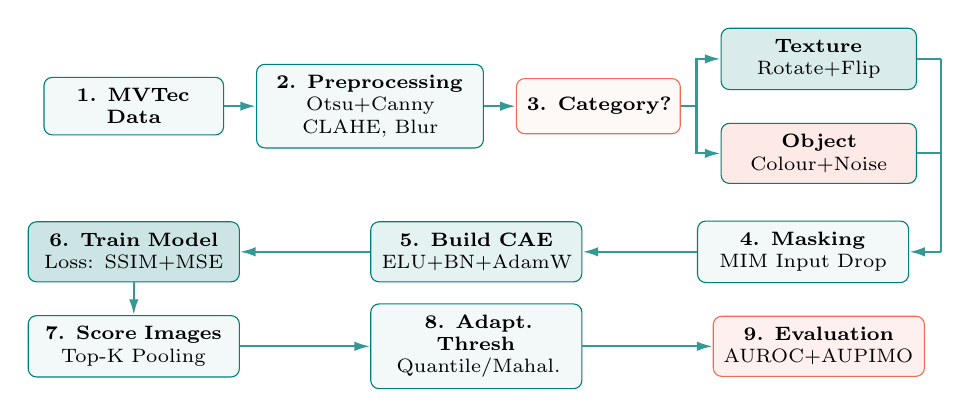
\begin{tikzpicture}[
  font=\scriptsize,
  stepbox/.style={draw=teal, fill=teal!5, rounded corners=3pt, text width=3.0cm, align=center, inner sep=4pt, minimum height=0.7cm},
  arr/.style={-{Latex[length=2mm,width=1.2mm]}, thick, color=teal!80}
]

  % ROW 1: Data Prep (L -> R)
  \node[stepbox, text width=2.0cm] (data) at (0, 0) {\textbf{1. MVTec Data}};
  \node[stepbox, text width=2.6cm] (prep) at (3.0, 0) {\textbf{2. Preprocessing}\\Otsu+Canny\\CLAHE, Blur};
  \node[stepbox, text width=1.8cm, fill=accent!5, draw=accent] (cat) at (5.9, 0) {\textbf{3. Category?}};
  \node[stepbox, text width=2.2cm, fill=teal!15] (tex) at (8.7, 0.6) {\textbf{Texture}\\Rotate+Flip};
  \node[stepbox, text width=2.2cm, fill=accent!15] (obj) at (8.7, -0.6) {\textbf{Object}\\Colour+Noise};

  \draw[arr] (data) -- (prep);
  \draw[arr] (prep) -- (cat);

  % Branching
  \draw[thick, color=teal!80] (cat.east) -- ++(0.2, 0) coordinate (fork);
  \draw[arr] (fork) |- (tex.west);
  \draw[arr] (fork) |- (obj.west);

  % ROW 2: Model (R -> L)
  \node[stepbox, text width=2.4cm, fill=teal!5] (mim) at (8.5, -1.85) {\textbf{4. Masking}\\MIM Input Drop};
  \node[stepbox, text width=2.4cm, fill=teal!10] (build) at (4.35, -1.85) {\textbf{5. Build CAE}\\ELU+BN+AdamW};
  \node[stepbox, text width=2.4cm, fill=teal!20] (train) at (0, -1.85) {\textbf{6. Train Model}\\Loss: SSIM+MSE};

  % Merge into MIM
  \draw[thick, color=teal!80] (tex.east) -- ++(0.3, 0) coordinate (tE); % codespell:ignore
  \draw[thick, color=teal!80] (obj.east) -- (tE |- obj.east) coordinate (oE); % codespell:ignore
  \draw[thick, color=teal!80] (tE) -- (oE); % codespell:ignore
  \draw[thick, color=teal!80] (oE) -- (tE |- mim.east) coordinate (mE); % codespell:ignore
  \draw[arr] (mE) -- (mim.east);

  \draw[arr] (mim) -- (build);
  \draw[arr] (build) -- (train);

  % ROW 3: Inference (L -> R)
  \node[stepbox, text width=2.4cm] (score) at (0, -3.05) {\textbf{7. Score Images}\\Top-K Pooling};
  \node[stepbox, text width=2.4cm] (thresh) at (4.35, -3.05) {\textbf{8. Adapt. Thresh}\\Quantile/Mahal.};
  \node[stepbox, text width=2.4cm, fill=accent!10, draw=accent] (eval) at (8.7, -3.05) {\textbf{9. Evaluation}\\AUROC+AUPIMO};

  \draw[arr] (train) -- (score);
  \draw[arr] (score) -- (thresh);
  \draw[arr] (thresh) -- (eval);

\end{tikzpicture}
}
\end{center}
\vspace{0.1cm}
{\textbf{\color{teal}Automated Pipeline \& Optuna Integration}\\
The pipeline is dynamically orchestrated. Hyperparameters (Preprocessing/Model) (e.g., augmentation strategy, latent dimensions) optimized using Optuna targeting \textbf{Pixel AUPIMO}.}
\note{\notefont
  \textbf{Q: Why optimise Optuna against AUPIMO and not AUROC?}\\[0.5pt]
  AUROC is threshold-free and integrates over the entire FPR range $[0,1]$.
  In industrial settings, operating at FPR $> 10^{-4}$ is practically useless
  (too many false alarms). AUPIMO evaluates \emph{only} the operationally relevant
  region and at pixel level, making it a far tighter proxy for real-world utility.
  Optimising AUROC could improve the broad curve while degrading the narrow
  high-stakes region that actually matters.\\[1.5pt]

  \textbf{Q: Why does Optuna target the validation split, not the test set?}\\[0.5pt]
  Any hyperparameter search against the test set is test leakage \emph{by design}.
  The 15\% normal validation partition (never anomalous, never test) is the only
  legal signal available for tuning. The test set is locked until final scoring.
  This is the ``zero-leakage'' guarantee \emph{within} the training process, not just
  a one-time split.\\[1.5pt]

  \textbf{Q: What does Optuna actually tune and how?}\\[0.5pt]
  Bayesian optimisation (Tree-structured Parzen Estimator) over the joint space of:
  crop size/stride, mask ratio, latent dimension, CLAHE clip limit, augmentation choice.
  It builds a probabilistic model of which configurations lead to high AUPIMO and
  samples the next trial from the most promising region. Far more efficient than
  grid/random search in high-dimensional spaces.\\[1.5pt]

  \textbf{Q: Why does the threshold calibration use the 95th percentile?}\\[0.5pt]
  It is a 5\% false-alarm budget on normal parts ($\alpha = 0.05$).
  This is the T2 ``Precision Industrial'' profile. 95\% of normal parts score below
  this threshold; 5\% are false positives. Setting $\alpha$ is the only
  available lever to control the false-alarm rate without defect labels.
  The key insight: this is a \emph{day-1 deployable SLA guarantee} on the false-alarm
  rate, even with zero knowledge of what defects look like.
}
\end{frame}

%====================================================================
%  SECTION: EVALUATION
%====================================================================
\section{Evaluation Protocol \& Benchmarks}

%--------------------------------------------------------------------
% SLIDE 10 – Fair Evaluation Split
%--------------------------------------------------------------------
\begin{frame}{Zero-Leakage Evaluation Protocol}
\begin{columns}[T]
  \begin{column}{0.50\textwidth}
    \textbf{The Core Principle}\\[8pt]
    {\small Every evaluation result in this presentation is produced under a
    deterministic, audit-compliant split that keeps the test set completely
    unseen until final scoring $\Rightarrow$ \textbf{zero-test-leakage}.}\\[8pt]
    
    \vspace{12pt}
    \textbf{Peak Performance (PatchCore vs CAE)}\\[4pt]
    \resizebox{0.95\linewidth}{!}{
      \begin{tabular}{llcc}
        \toprule
        \textbf{Category} & \textbf{Metric} & \textbf{PatchCore} & \textbf{Keras CAE} \\
        \midrule
        \multirow{2}{*}{Bottle (Object)} 
        & Image F1 & 0.962 & \textbf{0.992} \\
        & AUPIMO & \textbf{0.982} & 0.507 \\
        \midrule
        \multirow{2}{*}{Macro Average}
        & Image F1 & \textbf{0.929} & 0.495 \\
        & AUPIMO & \textbf{0.603} & 0.058 \\
        \bottomrule
      \end{tabular}
    }
  \end{column}
  \begin{column}{0.48\textwidth}
    \textbf{Canonical Evaluation Settings}\\[6pt]
    \begin{itemize}
      \item \textbf{Split Size:} 85\% fitting / 15\% validation
      \item \textbf{Test Set:} \textbf{held out} - normal + anomalies
      \item \textbf{Resolution:} $256 \times 256$ pixels.
        \begin{itemize}
          \item Bilinear interpolation for continuous heatmaps.
          \item Nearest-neighbor + binarization for GT masks.
        \end{itemize}
      \item \textbf{Threshold:} 95th percentile ($\alpha=0.05$ false-alarm budget).
      \item \textbf{AUPIMO:} Standard bounds $\text{FPR} \in [10^{-5}, 10^{-4}]$, 50k thresholds.
    \end{itemize}
  \end{column}
\end{columns}
\end{frame}

%--------------------------------------------------------------------
% SLIDE 11 – Side-by-Side Localisation Results
%--------------------------------------------------------------------
\begin{frame}{Qualitative Results - Localisation Comparison}
  \vspace{0.2cm}
  \begin{columns}[T]
    \begin{column}{0.16\textwidth}
      \centering
      \textbf{\scriptsize Input}
    \end{column}
    \begin{column}{0.16\textwidth}
      \centering
      \textbf{\scriptsize GT Mask}
    \end{column}
    \begin{column}{0.32\textwidth}
      \centering
      \textbf{\scriptsize \color{teal}PatchCore (Map \textbar{} Mask)}
    \end{column}
    \begin{column}{0.32\textwidth}
      \centering
      \textbf{\scriptsize \color{teal}Keras CAE (Map \textbar{} GT Overlay)}
    \end{column}
  \end{columns}
  
  \vspace{0.1cm}
  % Row 1: Bottle
  \begin{columns}[c]
    \begin{column}{0.16\textwidth}
      \centering
      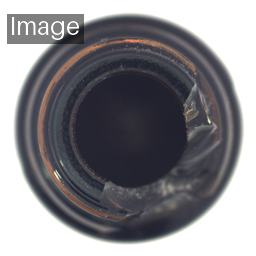
\includegraphics[width=0.9\linewidth]{figures/extracted/bottle/patchcore/original.png}
    \end{column}
    \begin{column}{0.16\textwidth}
      \centering
      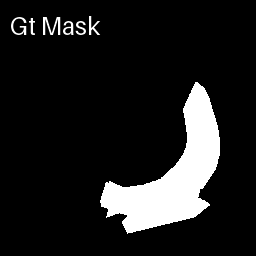
\includegraphics[width=0.9\linewidth]{figures/extracted/bottle/patchcore/gt_mask.png}
    \end{column}
    \begin{column}{0.32\textwidth}
      \centering
      
\includegraphics[width=0.45\linewidth]{figures/extracted/bottle/patchcore/anomaly_map.png}\hfill
      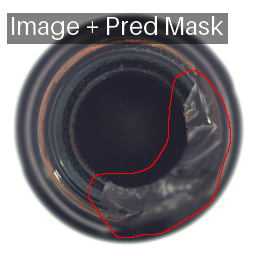
\includegraphics[width=0.45\linewidth]{figures/extracted/bottle/patchcore/predicted_mask.png}
    \end{column}
    \begin{column}{0.32\textwidth}
      \centering
      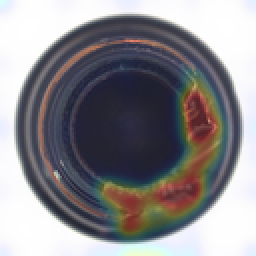
\includegraphics[width=0.45\linewidth]{figures/extracted/bottle/keras_cae/anomaly_map.png}\hfill
      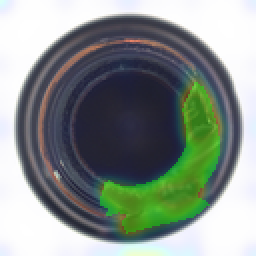
\includegraphics[width=0.45\linewidth]{figures/extracted/bottle/keras_cae/gt_overlay.png}
    \end{column}
  \end{columns}

  \vspace{0.1cm}
  % Row 2: Cable
  \begin{columns}[c]
    \begin{column}{0.16\textwidth}
      \centering
      
\includegraphics[width=0.9\linewidth]{figures/extracted/cable/patchcore/original.png}
    \end{column}
    \begin{column}{0.16\textwidth}
      \centering
      
\includegraphics[width=0.9\linewidth]{figures/extracted/cable/patchcore/gt_mask.png}
    \end{column}
    \begin{column}{0.32\textwidth}
      \centering
      
\includegraphics[width=0.45\linewidth]{figures/extracted/cable/patchcore/anomaly_map.png}\hfill
      
\includegraphics[width=0.45\linewidth]{figures/extracted/cable/patchcore/predicted_mask.png}
    \end{column}
    \begin{column}{0.32\textwidth}
      \centering
      
\includegraphics[width=0.45\linewidth]{figures/extracted/cable/keras_cae/anomaly_map.png}\hfill
      
\includegraphics[width=0.45\linewidth]{figures/extracted/cable/keras_cae/gt_overlay.png}
    \end{column}
  \end{columns}
  
  \vspace{0.2cm}
  \textbf{Key Observations:}
  \begin{itemize}
    \item \small \textbf{PatchCore:} Heatmaps sharply bound the defect, leading to precise predicted masks.
    \item \small \textbf{Keras CAE:} Reconstruction errors diffuse. While broadly highlighting anomalous regions, they fail at fine-grained pixel localization.
  \end{itemize}
\end{frame}

%====================================================================
%  SECTION: BUSINESS INTERPRETATION
%====================================================================
\section{Business Interpretation}

%--------------------------------------------------------------------
% SLIDE 11 – Economic Error Asymmetry
%--------------------------------------------------------------------
\begin{frame}{Economic Error Asymmetry}
  \textbf{A false alarm and a missed defect have different consequences.}\\[10pt]
  \begin{columns}[T,onlytextwidth]
    \begin{column}{0.47\textwidth}
      {\color{accent}\textbf{False alarm}}\\[4pt]
      A conforming part is flagged. Operators may need to inspect it again,
      slowing the line or creating scrap.\\[5pt]
      {\small\color{muted}Throughput-sensitive lines may put greater weight on this cost.}
    \end{column}
    \begin{column}{0.47\textwidth}
      {\color{teal}\textbf{Missed defect}}\\[4pt]
      A defective part passes inspection. Downstream rework, warranty claims,
      recalls or safety risks may follow.\\[5pt]
      {\small\color{muted}High-consequence applications may put greater weight on this cost.}
    \end{column}
  \end{columns}
  \vspace{16pt}
  \begin{center}
    $C(\tau)=c_{\mathrm{FP}}\,\mathrm{FP}(\tau)+c_{\mathrm{FN}}\,\mathrm{FN}(\tau)$\\[6pt]
    {\small\color{muted}A decision framework: plant-specific costs and error counts must be measured before choosing a gate.}
  \end{center}
\end{frame}

%--------------------------------------------------------------------
% SLIDE 12 – Threshold Calibration & Risk Tiers
%--------------------------------------------------------------------
\begin{frame}{Threshold Calibration \& Operating Priorities}
  \begin{columns}[T,onlytextwidth]
    \begin{column}{0.47\textwidth}
      \textbf{Normal-validation calibration}\\[4pt]
      {\footnotesize Cost priorities guide the choice of $\alpha$; normal scores turn it into $\tau_\alpha$.}\\[6pt]
      {\small\mbox{$\tau_\alpha = \operatorname{Quantile}_{1-\alpha}
      \left(\mathrm{AnomalyScores}_{\mathrm{normal,val}}\right)$}}\\[6pt]
      {\small $\alpha$ is a budget on held-out normal data,
      not a production guarantee.}\\[6pt]
      {\small\textbf{Proposed priorities}}\\[3pt]
      {\small\color{accent}Recall priority} ($\alpha\approx0.10$): lower gate, more review.\\[3pt]
      {\small\color{teal}Balanced starting point} ($\alpha=0.05$): reported benchmark setting.\\[3pt]
      {\small\color{muted}Throughput priority} ($\alpha\approx0.01$): higher gate, fewer flags on normal validation data.
    \end{column}
    \begin{column}{0.51\textwidth}
      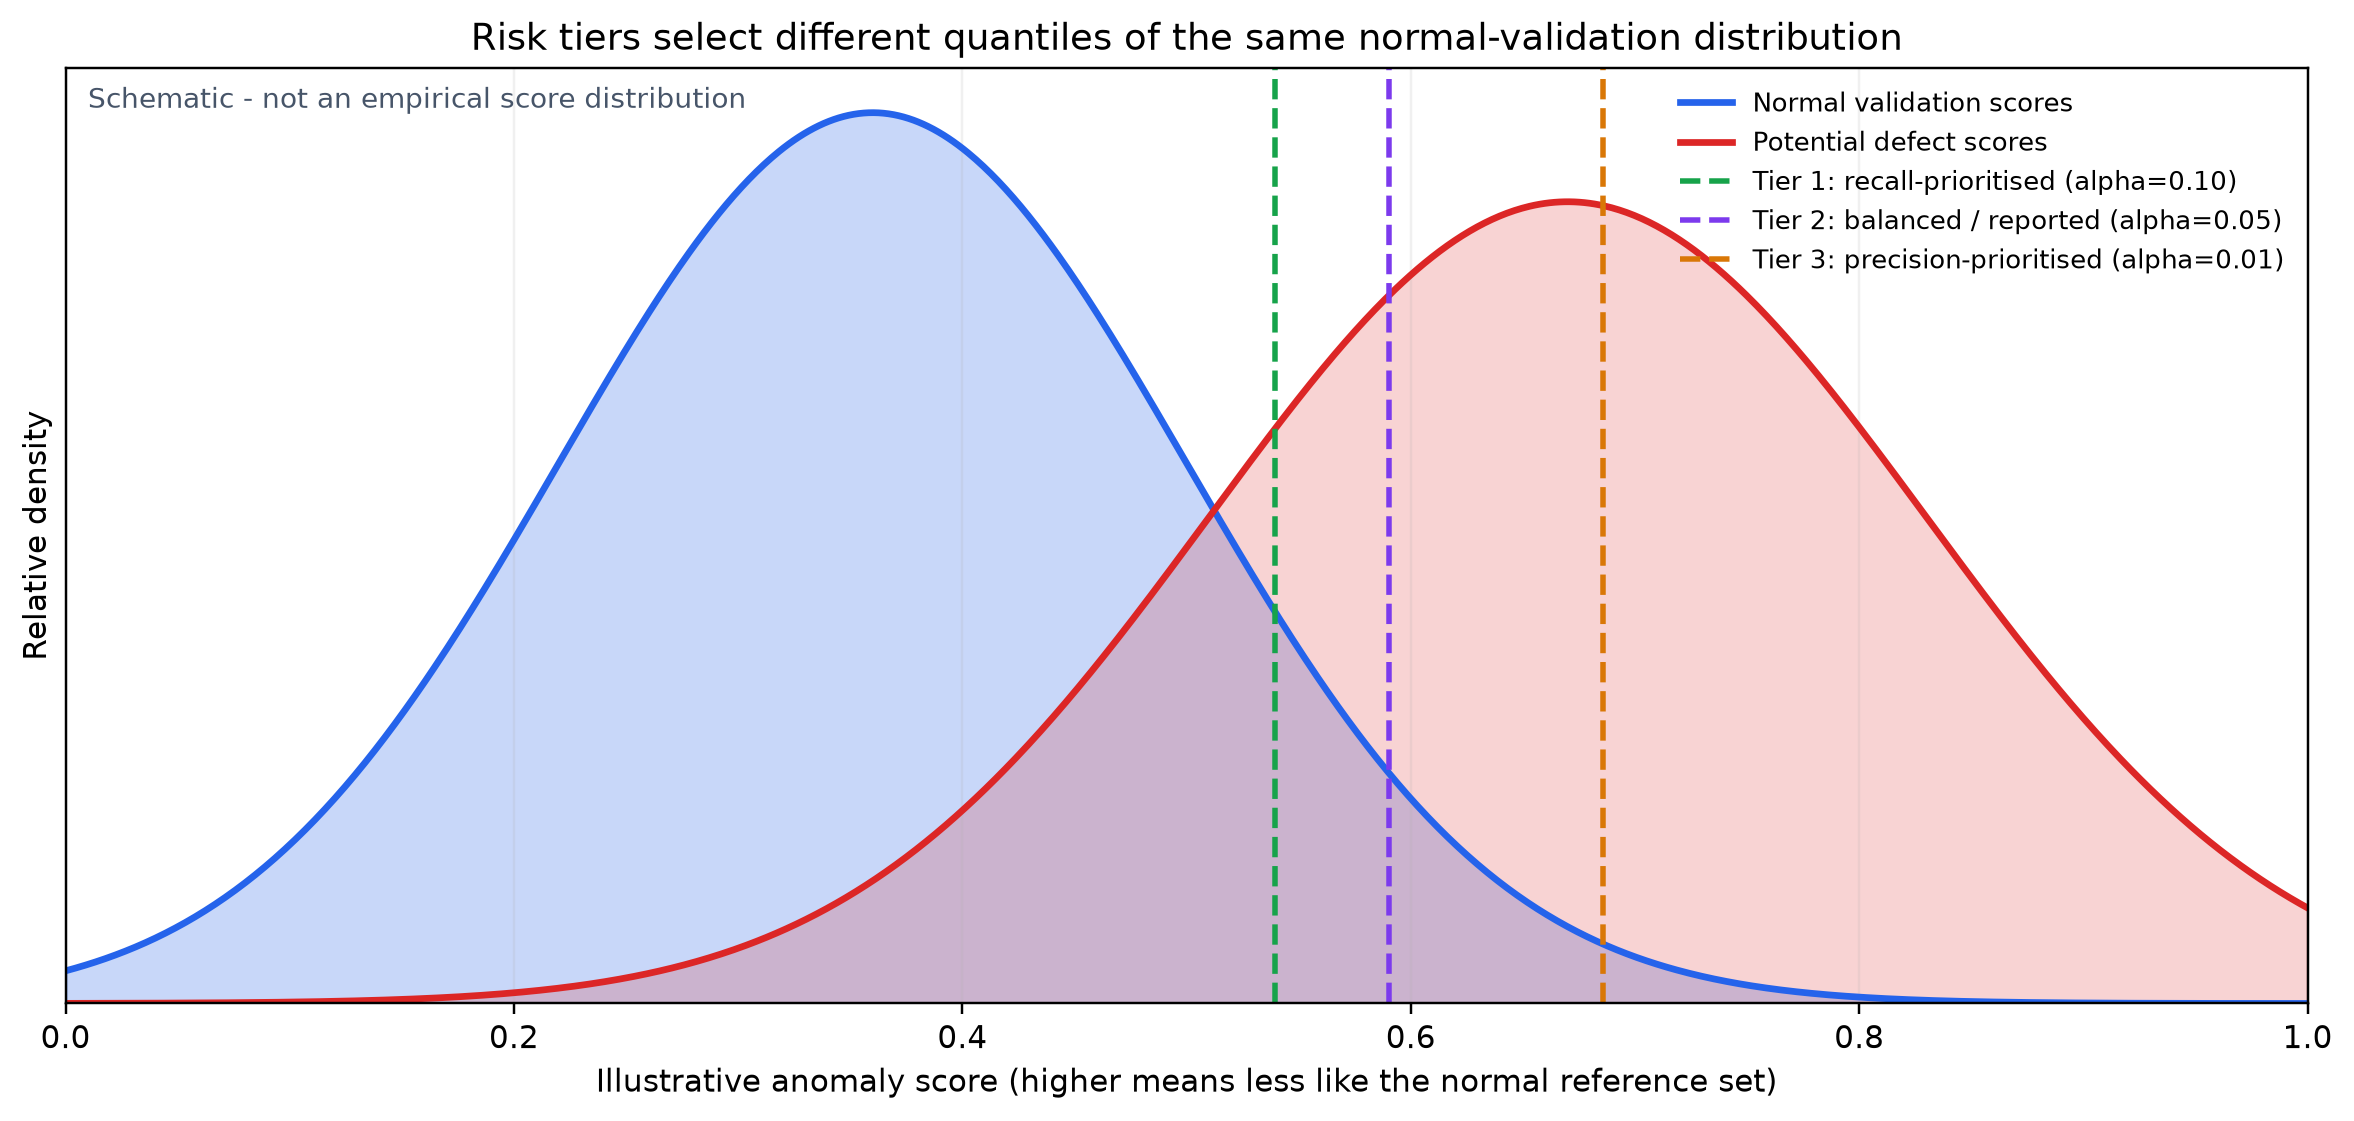
\includegraphics[width=\textwidth]{business_threshold_tiers.png}\\[5pt]
      {\footnotesize\color{muted}Schematic only. Defect recall and real-line false alarms
      must be checked with plant data for each proposed setting.}
    \end{column}
  \end{columns}
\end{frame}

%--------------------------------------------------------------------
% SLIDE 13 – Operator Evidence
%--------------------------------------------------------------------
\begin{frame}{Operator Evidence for Review}
  \textbf{A flagged image needs visible evidence and a human decision path.}\\[8pt]
  \begin{columns}[T,onlytextwidth]
    \begin{column}{0.31\textwidth}
      \centering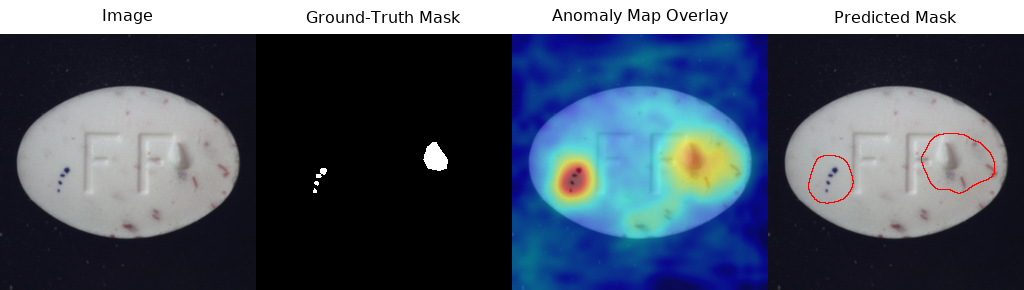
\includegraphics[viewport=0bp 0bp 256bp 256bp,clip,width=0.70\linewidth]{figures/business/pill_patchcore_003.png}\\[3pt]
      {\small Input image}
    \end{column}
    \begin{column}{0.31\textwidth}
      \centering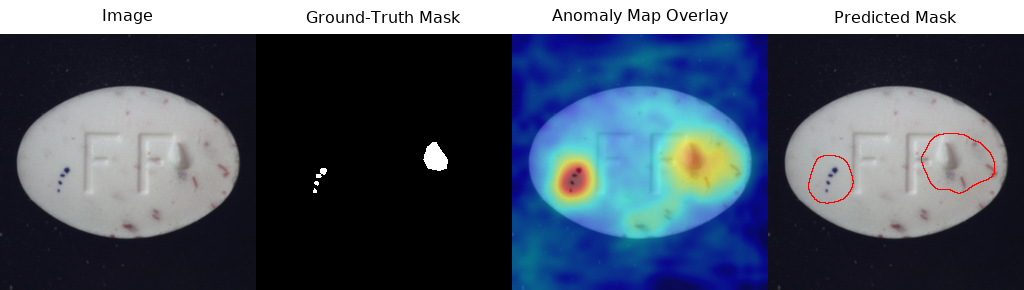
\includegraphics[viewport=512bp 0bp 768bp 256bp,clip,width=0.70\linewidth]{figures/business/pill_patchcore_003.png}\\[3pt]
      {\small Anomaly map}
    \end{column}
    \begin{column}{0.31\textwidth}
      \centering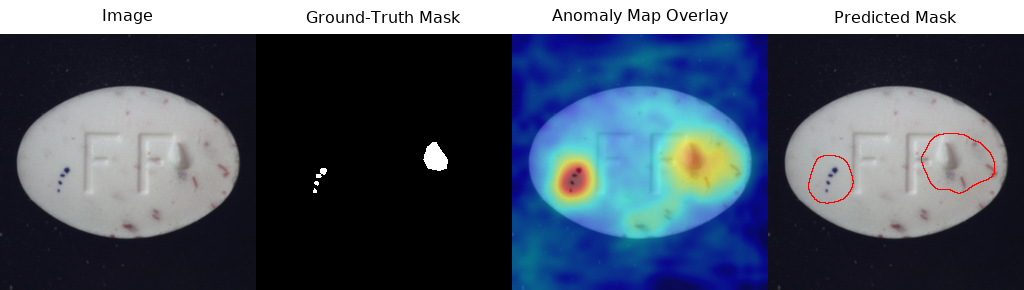
\includegraphics[viewport=768bp 0bp 1024bp 256bp,clip,width=0.70\linewidth]{figures/business/pill_patchcore_003.png}\\[3pt]
      {\small Predicted contour}
    \end{column}
  \end{columns}
  \vspace{4pt}
  {\footnotesize\color{muted}PatchCore highlights suspected defect regions; the heatmap does not establish the cause.}\\[5pt]
  {\small Borderline flags should go to quality engineers for review during a controlled pilot.
  Review time and operator agreement still need measurement.}
\end{frame}

%--------------------------------------------------------------------
% SLIDE 14 – Team Conclusion
%--------------------------------------------------------------------
\begin{frame}{Conclusion \& Next Steps}
  \begin{columns}[T,onlytextwidth]
    \begin{column}{0.47\textwidth}
      \textbf{\color{teal}What We Demonstrated}
      \begin{itemize}\small
        \setlength{\itemsep}{7pt}
        \item EDA revealed the limitations of conventional evaluation metrics.
        \item Developed and compared convolutional autoencoders and PatchCore.
        \item Established a consistent evaluation and threshold-calibration framework.
      \end{itemize}
    \end{column}
    \begin{column}{0.47\textwidth}
      \textbf{\color{teal}What Comes Next}
      \begin{itemize}\small
        \setlength{\itemsep}{7pt}
        \item Validate on representative production data.
        \item Calibrate thresholds against plant-specific risks.
        \item Run a controlled industrial pilot before deployment.
      \end{itemize}
    \end{column}
  \end{columns}
  \vspace{4pt}
  {\small\centering From understanding defects to building a model, and from model performance to industrial decisions.\par}
  \vspace{2pt}
  \begin{center}
    \fcolorbox{teal}{teal!8}{%
      \parbox{0.48\textwidth}{\centering\vspace{2pt}
        {\large\bfseries\color{teal}Thank you}\\[1pt]
        {\small Questions \& Discussion}\\[2pt]
        {\footnotesize\color{muted}B.~Förster $\cdot$ A.~Abul~Hawa\\
        M.~Nadaf $\cdot$ K.~Khalifa}\vspace{2pt}}
    }
  \end{center}
\end{frame}

\end{document}
